\documentclass{article}
\usepackage{a4}
\usepackage{hyperref}
\usepackage{graphicx}
\usepackage{listings}
\usepackage{tabularx}
\usepackage{pifont}

\begin{document}

\title{Exploring Machine Learning:\\
  The ID3 algorithm\\
  		Testing Document}


\author{Mohammed Ibrahim\\
 Computer Science Department\\
  College of Science, Swansea University\\
  Swansea, SA2 8PP, UK
}
\pagebreak

\maketitle

\abstract{This document discuss the different types of testing we have used namely Junit testing and V- Model. It also includes the screen shots in which the information gain was calculated to select the root node. The test suite are described in the tabular format according to our specification code. }
\pagebreak

\tableofcontents
\pagebreak

\section{Introduction}
\label{sec:intro}


We have used two different testing methodologies for this Machine learning project; Junit testing and V-model. Initially we have started with Junit testing, Eclipse supports Junit testing, it is a method by which individual units of source code are tested to determine if they are fit for use. We initially started compiling test cases for each function, we added and tested over all programs. The V-model represents a software development process this model is an extension of water fall model. Instead of moving down in a linear way, the process steps are bent upwards after the coding phase, to form the typical V shape. The V-Model demonstrates the relationships between each phase of the development life cycle and its associated phase of testing. V-model is that unlike the waterfall model.

\section{V-Model Testing}
 \label{sec:vmod}

The V model is a modified version of the water fall model. In the initial document I have describe that I will use waterfall model later I find the identical model, modified version of water fall model called V-model. 

V model has very stages:

\subsection{Requirement analysis :}

Requirement analysis is the first step in the verification process. In this stage we decide the projects and its function. During this stage I have discussed with my supervisor how the program is going to be created. So, we decided to create to different types of Java programs one is called `ComputeDecisionTree'' and other is called the `ApplyDecisionTree''. \\
In this stage we also planned to create different phases.

\begin{itemize}

\item {\bf Phase 1: Implementation} During this phase two programs are created {\bf ``ComputeDecisionTree"} and {\bf ``ApplyDecisionTree "}.

\item {\bf Phase 2: Thorough testing, and additional documentation}
During this phase we have submitted the interim document, In the interim document precisely explained input and output file format, but testing we have done after the completion of each program.

\item {\bf Phase 3: Evaluation} During this phase training sets are evaluated. Details about the evaluation can find in the reflective document. 


\end{itemize}

\subsection{System Design}

During this stage possible design of the program was formulated. We decided to specify the input file format and out put file format. 

\subsection{Architecture Design}

The architecture design is also known as software design it realizes the modules and the functionality of modules which have to be incorporated. In our program we have not use any types of GUI.
 
\subsection{Module Design} 
In the module design, the architectural design is again broken up into sub units so that they can be studied and explained separately. The units are called modules. The modules can separately be decoded by the programmer. 
 
\section{Unit testing (JUnit)}
\label{sec:junit}

According to the book of \cite{Jones1990SoftwareEngineering}(page 392, Chapter 8): Unit testing : It is the process of taking a program module and running it in isolation from the rest of the software by using prepared input and comparing the actual results with the results  predicted by the specifications and design of the module. The main purpose of testing is to find and debug the errors in the program.\\
There are three main reasons for unit testing :
\begin{enumerate}
\item The size of a single module is small enough that we can locate an error fairly easily.
\item Confusing interactions of multiple errors in widely different parts of the software are eliminated.
\item The module is small enough that we can attempt to test it in some demonstrably exhaustive fashion.
\end{enumerate}
To refer from \cite{JUnitTestingUtilityTutorial}(page 1): JUnit is a framework which helps to test, debug and implement the program in Java. It provides a simple way to explicitly test specific areas of a Java program, it is extensible and can be employed to test a hierarchy of program code either singularly or as multiple units.

JUnit helps the idea of first testing then coding, in that it is possible to setup test data for a unit which defines what the expected output is and then code until the tests pass. It is believed by some that this practice of "test a little, code a little, test a little, code a little..." increases programmer productivity and stability of program code whilst reducing programmer stress and the time spent debugging

According to \cite{JUnitTestingUtilityTutorial}(page 1): JUnit helps first testing then coding, in the program it is possible to arrange the test data for a unit which defines what the expected output is and then code until the tests pass.\\
In our project the program will be tested and implemented same time using JUnit testing.  
\pagebreak

\section{Testing File format }

The file format was important for testing in this program. There are two types of file format we valid file format and invalid file format. 
When we consider the data sets our first work is to test the data set, whether the data set is according to our specified file format or not. If the data set is valid, we input the file to get the decision tree.  
\section{Testing Attributes}

Testing the attributes is very important as to select the root node. We chose the root node for that attributes which has highest information gain. In our case the outlook information has highest information compare with other three attributes. I have worked out(calculate) all the four attributes to know the information gain as to select the root node.
The below screen shots shows the calculation of information gain: Briefly explained about information gain int narrative and reflective document. Here, we have tested which attributes to select as root node.
{\bf Gain(S, Outlook) =0.246}\\
{\bf Gain(S, Humidity) =0.151}\\
{\bf Gain(S, Wind) = 0.048}\\
{\bf Gain(S, Temperature) = 0.029}\\
We have selected Outlook attributes as a root node because it has highest information gain. 


\pagebreak
\begin{figure}[hbtp]
\centering
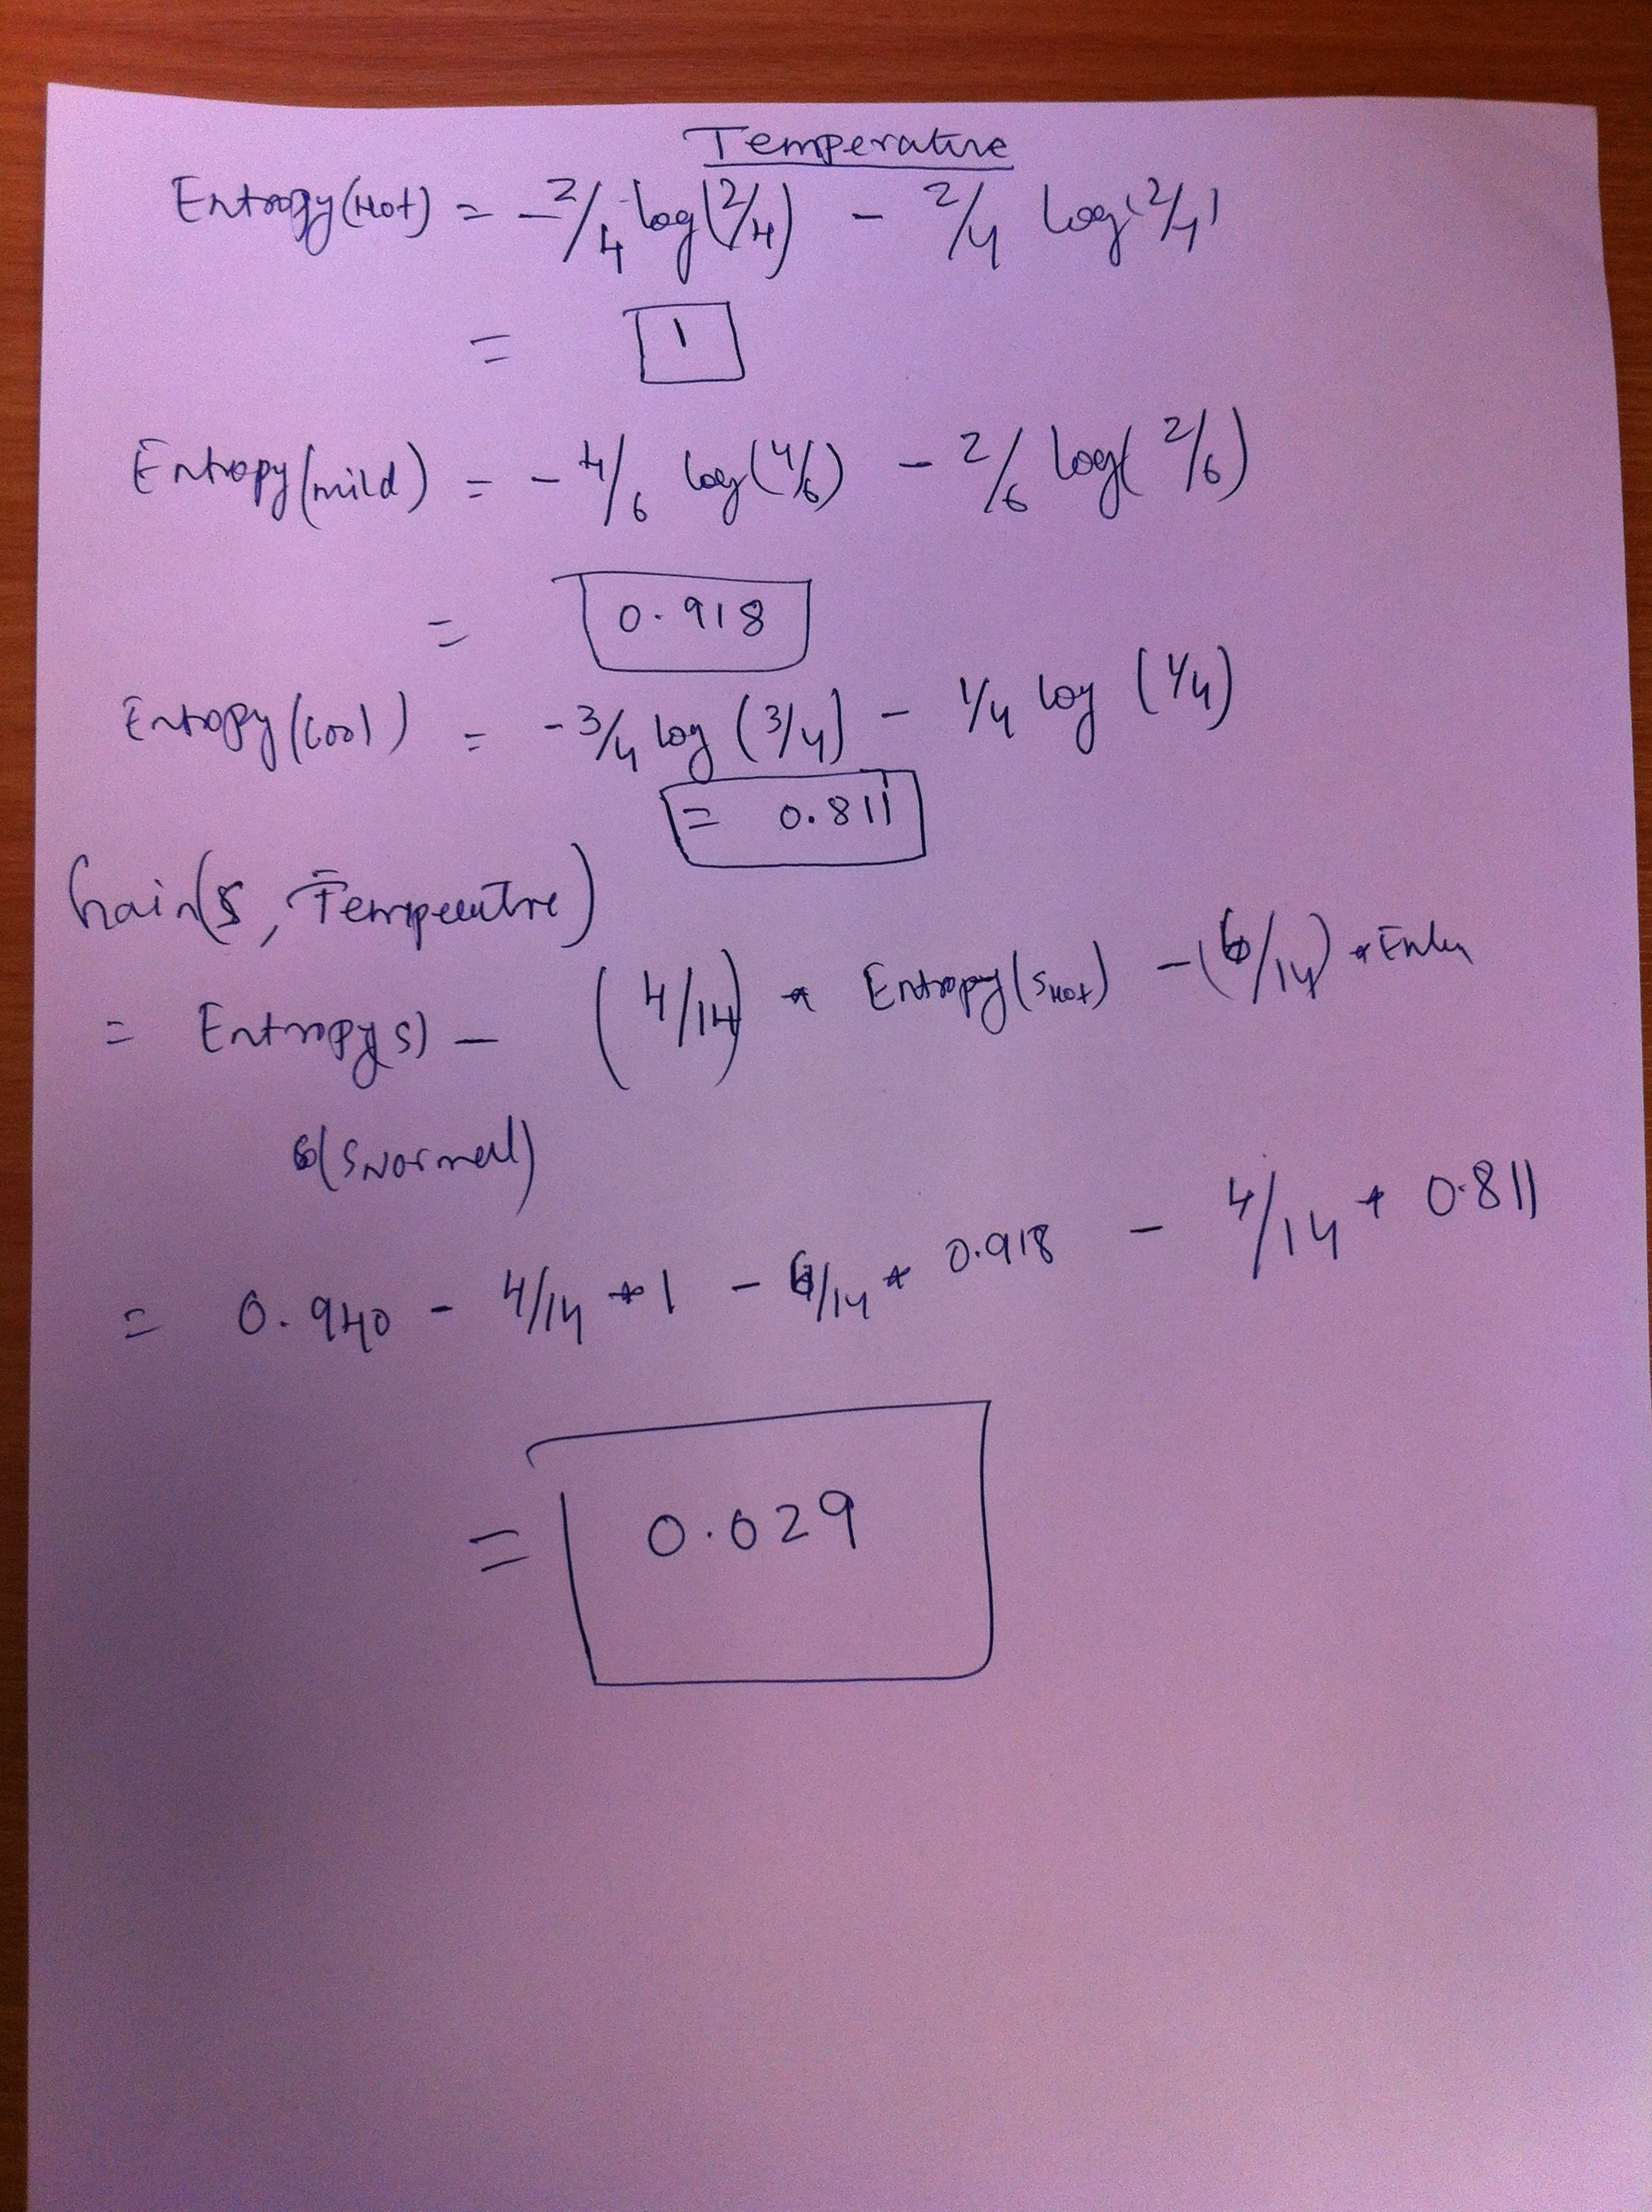
\includegraphics[scale=0.2]{IMG_0733.jpg}
\caption{Temperature}
\end{figure}

\begin{figure}[hbtp]
\centering
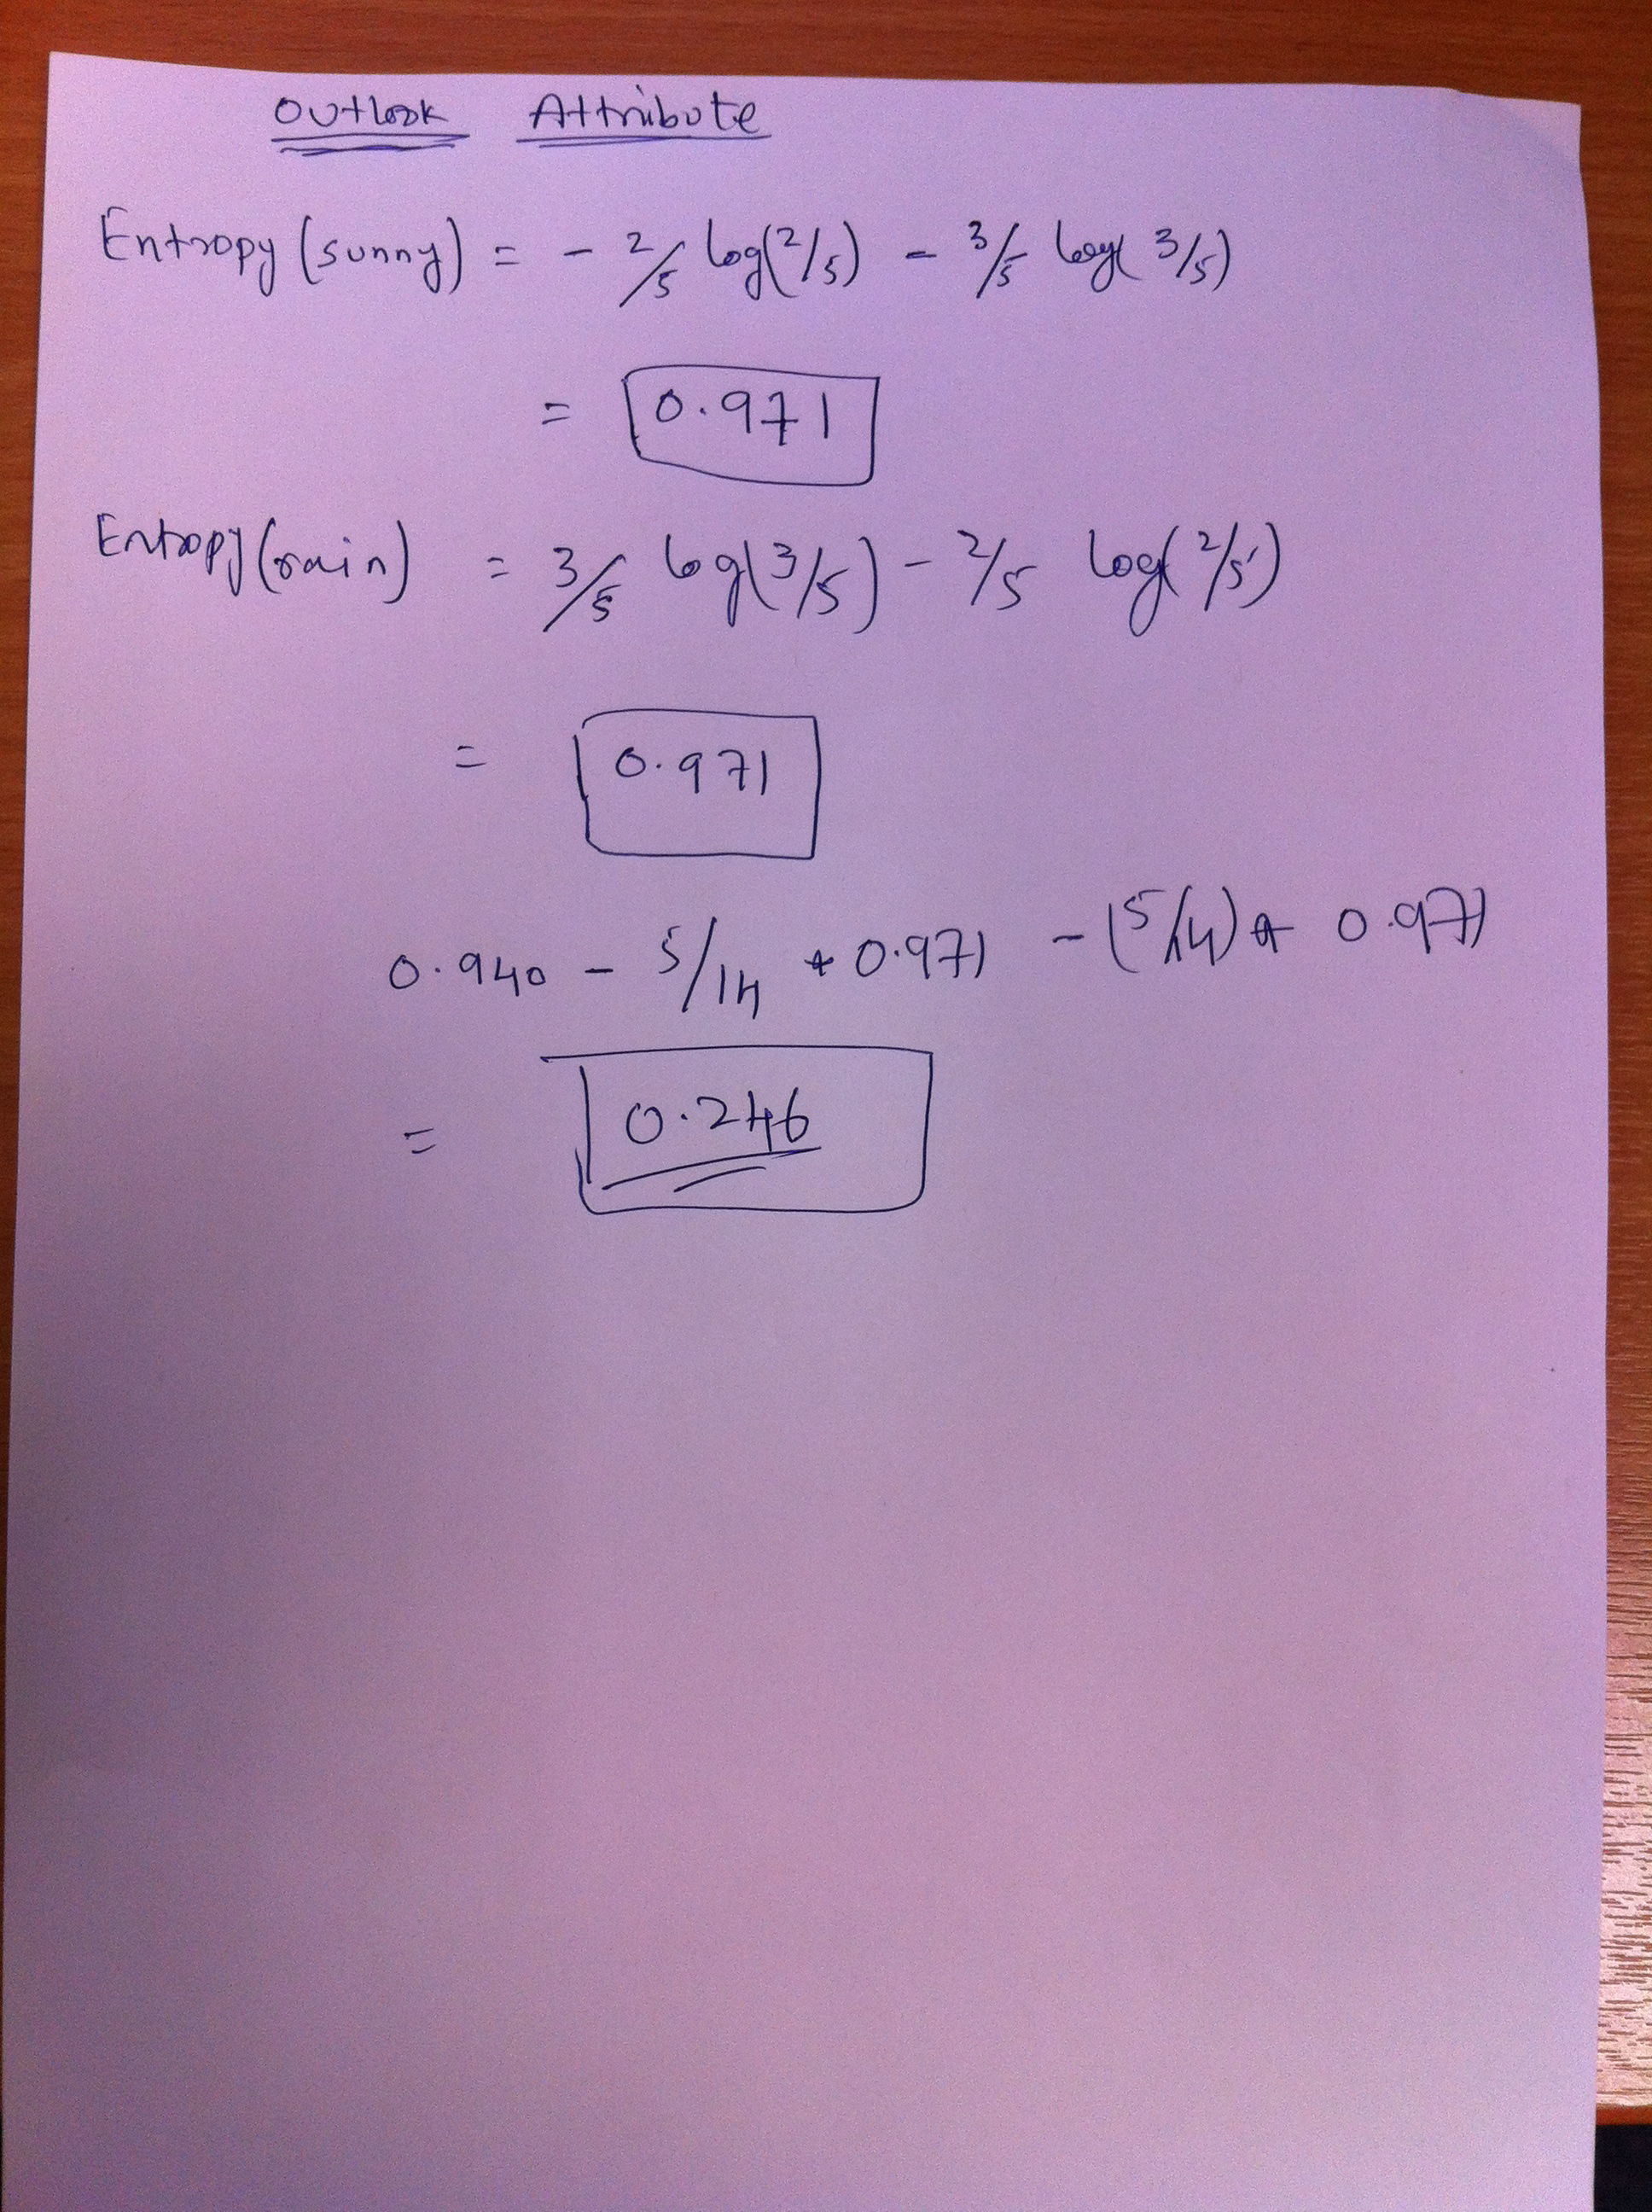
\includegraphics[scale=0.2]{IMG_0734.JPG}
\caption{Outlook}
\end{figure}

\begin{figure}[hbtp]
\centering
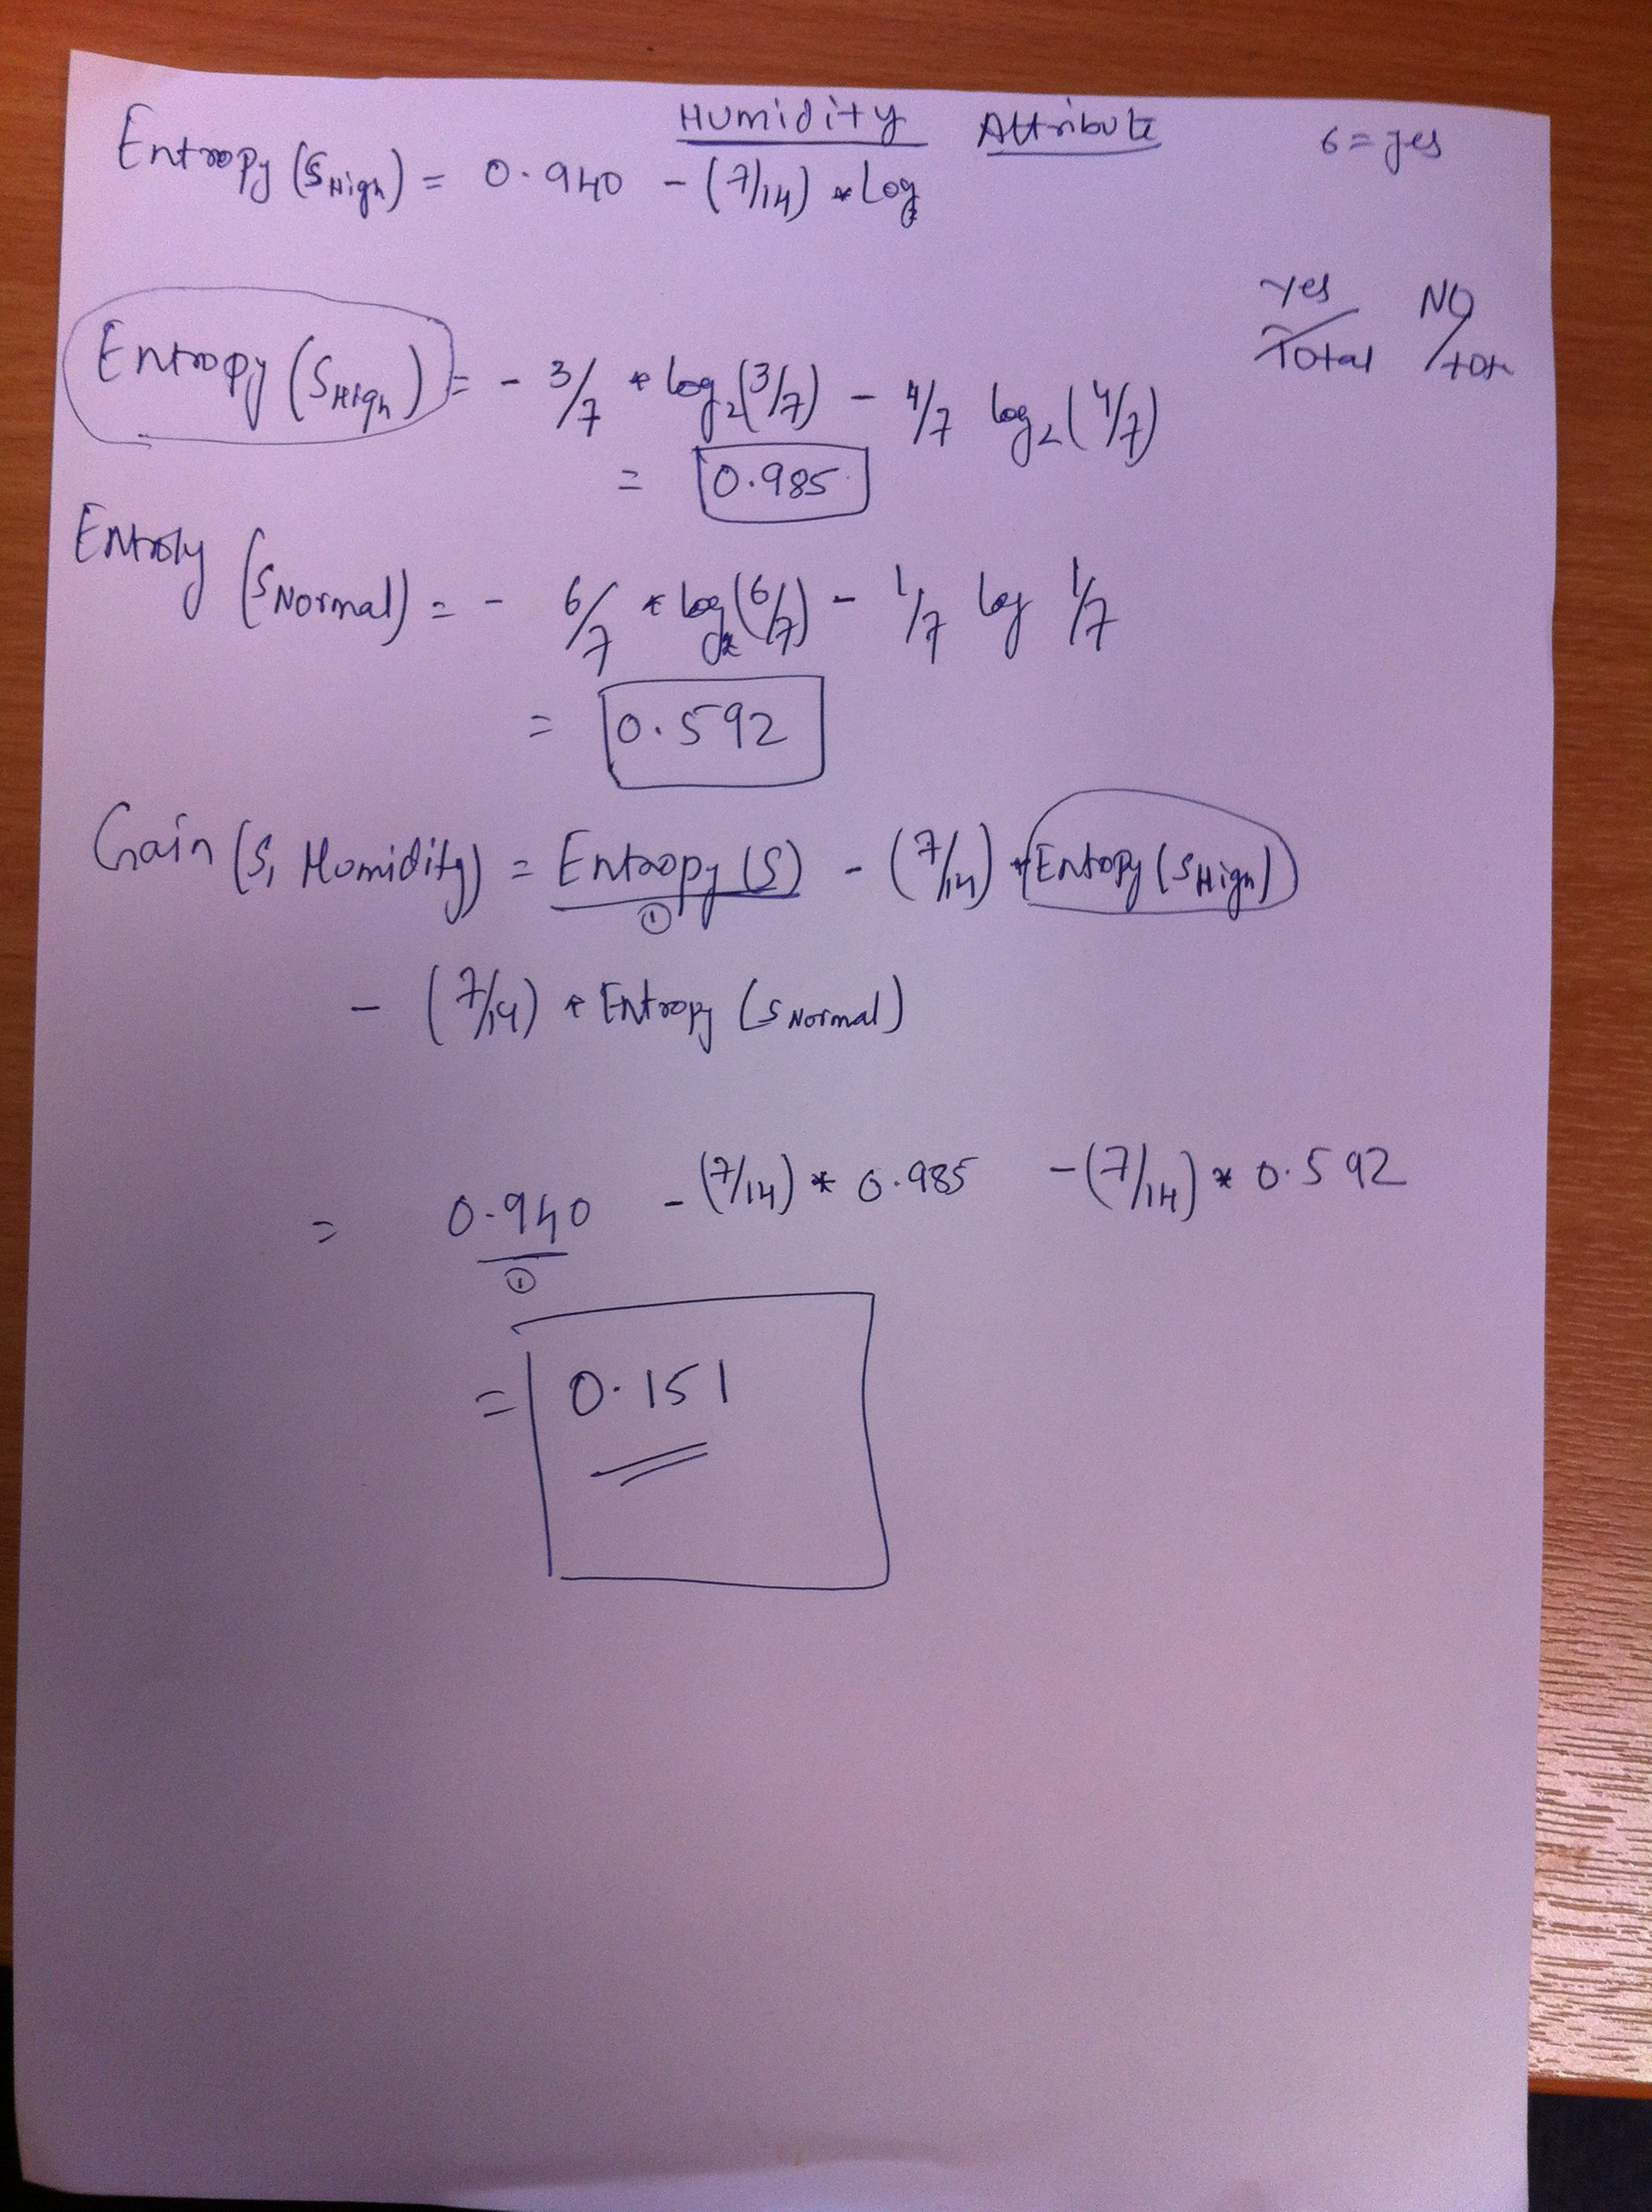
\includegraphics[scale=0.2]{IMG_0735.JPG}
\caption{Humidity}
\end{figure}

\newpage


\section{Test Suite}
\label{sec:test}
\begin{table}[ht]
\caption{Test Cases for Specification} 
\centering
\begin{tabularx}{\textwidth}{|l|X|X|l|l|X|} 
\hline \hline 
Id & Test Name & Description & Spec & Result & Comment \\ 
\hline \hline 
1 & Java application produce two sets of programs & First program computes Decision tree second program apply decision tree & SPEC1 & Pass & N/A \\\hline 
2 & Input training sets file & The program allows user to input the training sets file & SPEC2 & Pass & File could be valid or invalid \\\hline
3 & Check input file format & data sets have to be in a specified file format & SPEC3 & Pass & N/A\\\hline
4 & Comments ignore & Comments are ignored in the data sets & SPEC4 & Pass & N/A \\\hline
5 & Check blank line in training set file & All the blank line will be ignored in the training set file & SPEC5 & Pass & N/A \\\hline
6 & Attributes,values separated by single space & All the attributes and values are separated by using single space & SPEC6 & Pass & N/A \\\hline 

\end{tabularx}
\end{table}
\pagebreak

\begin{table}[ht]
\caption{Test Cases for Specification} 
\centering
\begin{tabularx}{\textwidth}{|l|X|X|l|l|X|} 
\hline \hline 
Id & Test Name & Description & Spec & Result & Comment \\ 
\hline \hline 

7 & First recognizable line of the data file have to be an attributes. & The very first recognizable line of the data file have to be an attributes & SPEC7 & Pass & N/A \\\hline 
9 & Target attribute & The last word of the attribute is taken as the target attribute in the data training sets. & SPEC8 & Pass & N/A \\\hline 
10 & Output the Decision tree & The program produce the Decision tree in a separate file  & SPEC9 & Pass & N/A \\\hline 
11 & Statistics & The second file will produce the statistics that corresponds to the algorithms implemented. & SPEC10 & Fail & The program only shows the size of the table \\\hline
12 & Validation set & The second program checks validation set and output the target attribute & SPEC11 & pass & N/A \\\hline
13 & Check error rate & Second program produce the error rate & SPEC12 & Pass & N/A \\\hline


\end{tabularx}
\end{table}
\pagebreak


\bibliographystyle{plain}
\bibliography{Bibliography}



\end{document}